\section{Задание 2. Площадь фигуры}
\subsection*{Задание}
Найдите площадь фигуры, ограниченной кривой Лиссажу $x = 2sint$, $y = 2sin2t$
\subsection*{График кривой:}
\begin{center}
	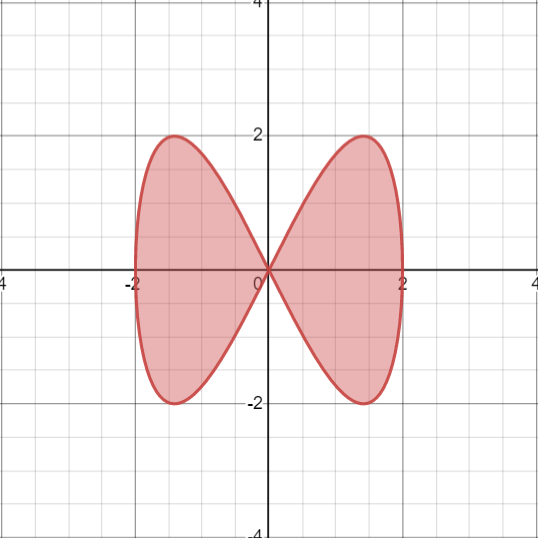
\includegraphics[width=0.4\linewidth]{task2_img1}\\
	\url{https://www.desmos.com/calculator/2y0dajpihq}
\end{center}
Кривая симметрична относительно обеих осей координат: если заменить $t$ на $(\pi - t)$, то переменная x не меняется, a $y$ изменяет только свой знак;
следовательно, кривая симметрична относительно оси $Ox$. При замене же $t$ на $(\pi + t)$ переменная $y$ не меняется, а $x$ меняет только свой знак. Это значит, что кривая симметрична относительно оси $Oy$.

В силу симметричности фигуры, для нахождения ее площади достаточно рассмотреть только четверть, значение на отрезке $[0, \frac{\pi}{2}]$ 
\begin{center}
	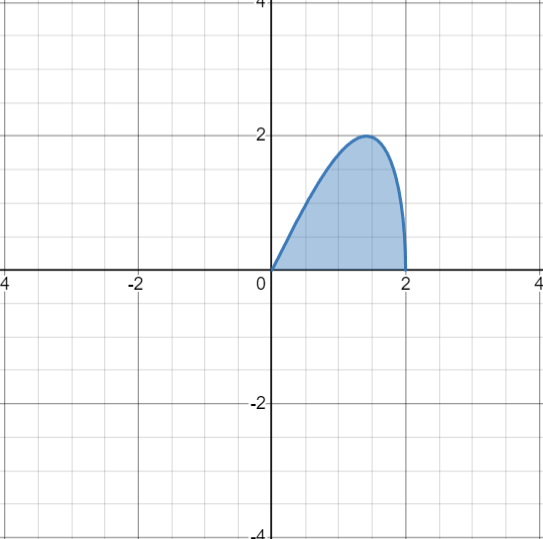
\includegraphics[width=0.4\linewidth]{task2_img2}\\
\end{center}

Тогда искомая
площадь будет равна полученному результату, умноженному на 4:\\
$S = 4 \int\limits_0^{\frac{\pi}{2}} y(x) x_t 'dt = 4 \int\limits_0^{\frac{\pi}{2}} 2 \cdot sin2t \cdot 2 \cdot cost dt = 16 \int\limits_0^{\frac{\pi}{2}} 2 \cdot sint \cdot cos^{2}t dt = -32 \int\limits_0^{\frac{\pi}{2}} cos^{2}t d(cost) = -32 \cdot {\frac{cos^{3}t}{3}} \bigg|_0^{\frac{\pi}{2}} = {\frac{32}{3}}$ 